\documentclass[a4paper]{article}

\usepackage{Template}

%标题部分
\newcommand\theheader{\LaTeX 模板}
\newcommand\thefooter{小臣子吃大橙子 \texttt{JamesZhutheThird@vip.qq.com}}

\title{\LaTeX 模板}
\author{JamesZhutheThird}
\date{\today}
%\date{YYYYMMDD}

\begin{document}
\maketitle
\pagestyle{fancyStyle}
\thispagestyle{fancyStyleForTitle}
%\thispagestyle{fancyStyleForTitleNoLogo} %用于隐藏校徽

%摘要部分
\begin{abstract}
摘要摘要摘要摘要摘要摘要摘要摘要摘要摘要摘要摘要摘要摘要摘要摘要摘要摘要摘要摘要摘要摘要摘要摘要摘要摘要\textbf{关键字}摘要摘要摘要摘要摘要摘要摘要摘要摘要摘要摘要摘要摘要摘摘要摘要摘要摘要摘要摘要摘要摘要摘要摘要摘要摘要摘要摘要要摘要摘要摘要摘要摘要摘要摘要摘要摘要摘要摘要摘要摘要摘要摘要摘要\textbf{关键字}摘要摘要摘要摘要摘要摘要摘要摘要摘要摘要\textbf{关键字}摘要摘要摘要摘要摘要摘要摘要\textbf{关键字}摘要摘要摘要摘要摘要摘要摘要摘要摘要摘要摘要摘要摘要摘要摘要摘要摘要
\par\textbf{关键字:}关键字,关键字,关键字,关键字
\end{abstract}


\section{模板}
\subsection{插入图片}
\subsubsection{单张图片}
正文正文正文正文正文正文正文正文\cite{doi:10.5772/4740}正文正文正文正文正文正文正文正文正文正文正文正文正文正文正文正文正文正文正文正文正文正文正文正文正文正文正文正文正文正文正文正文正文正文正文正文正文正文正文正文正文正文正文正文正文正文正文正文正文正文正文正文正文正文正文正文正文正文正文正文正文正文正文正文如图\ref{fig:single}\ref{fig:pdf}\ref{fig:svg}所示

\begin{figure}[!h]
	\centering
	\vspace{0cm}
	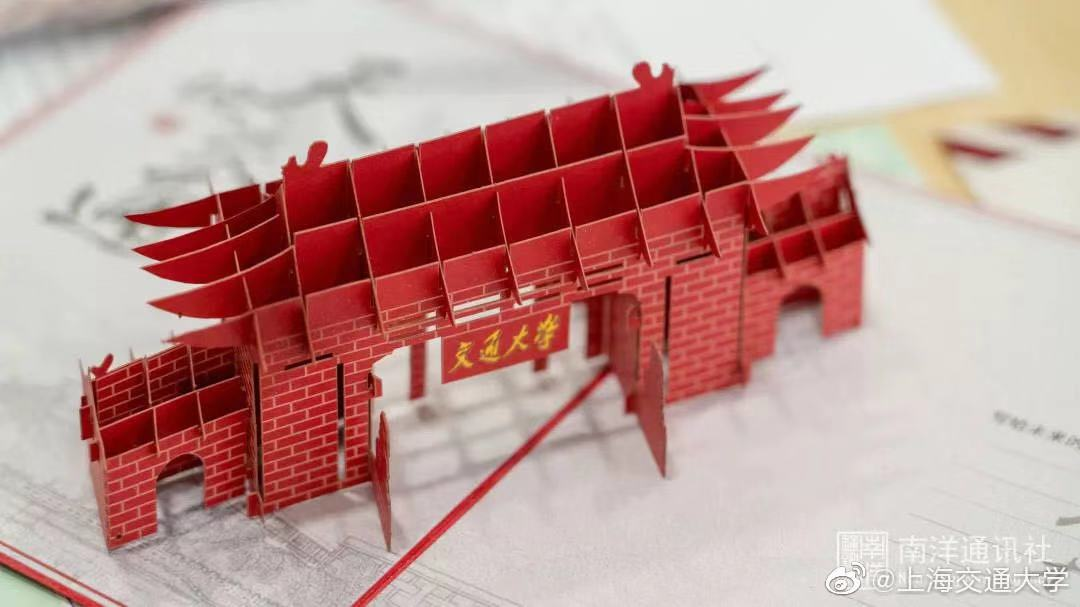
\includegraphics[width=0.4\textwidth,trim=50 100 200 75,clip]{figures/fig1.jpg}%trim裁切依次左下右上
	\vspace{0cm}
	\caption{图标题}
	\label{fig:single}
\end{figure}

\begin{figure}[!h]
	\centering
	\vspace{0cm}
	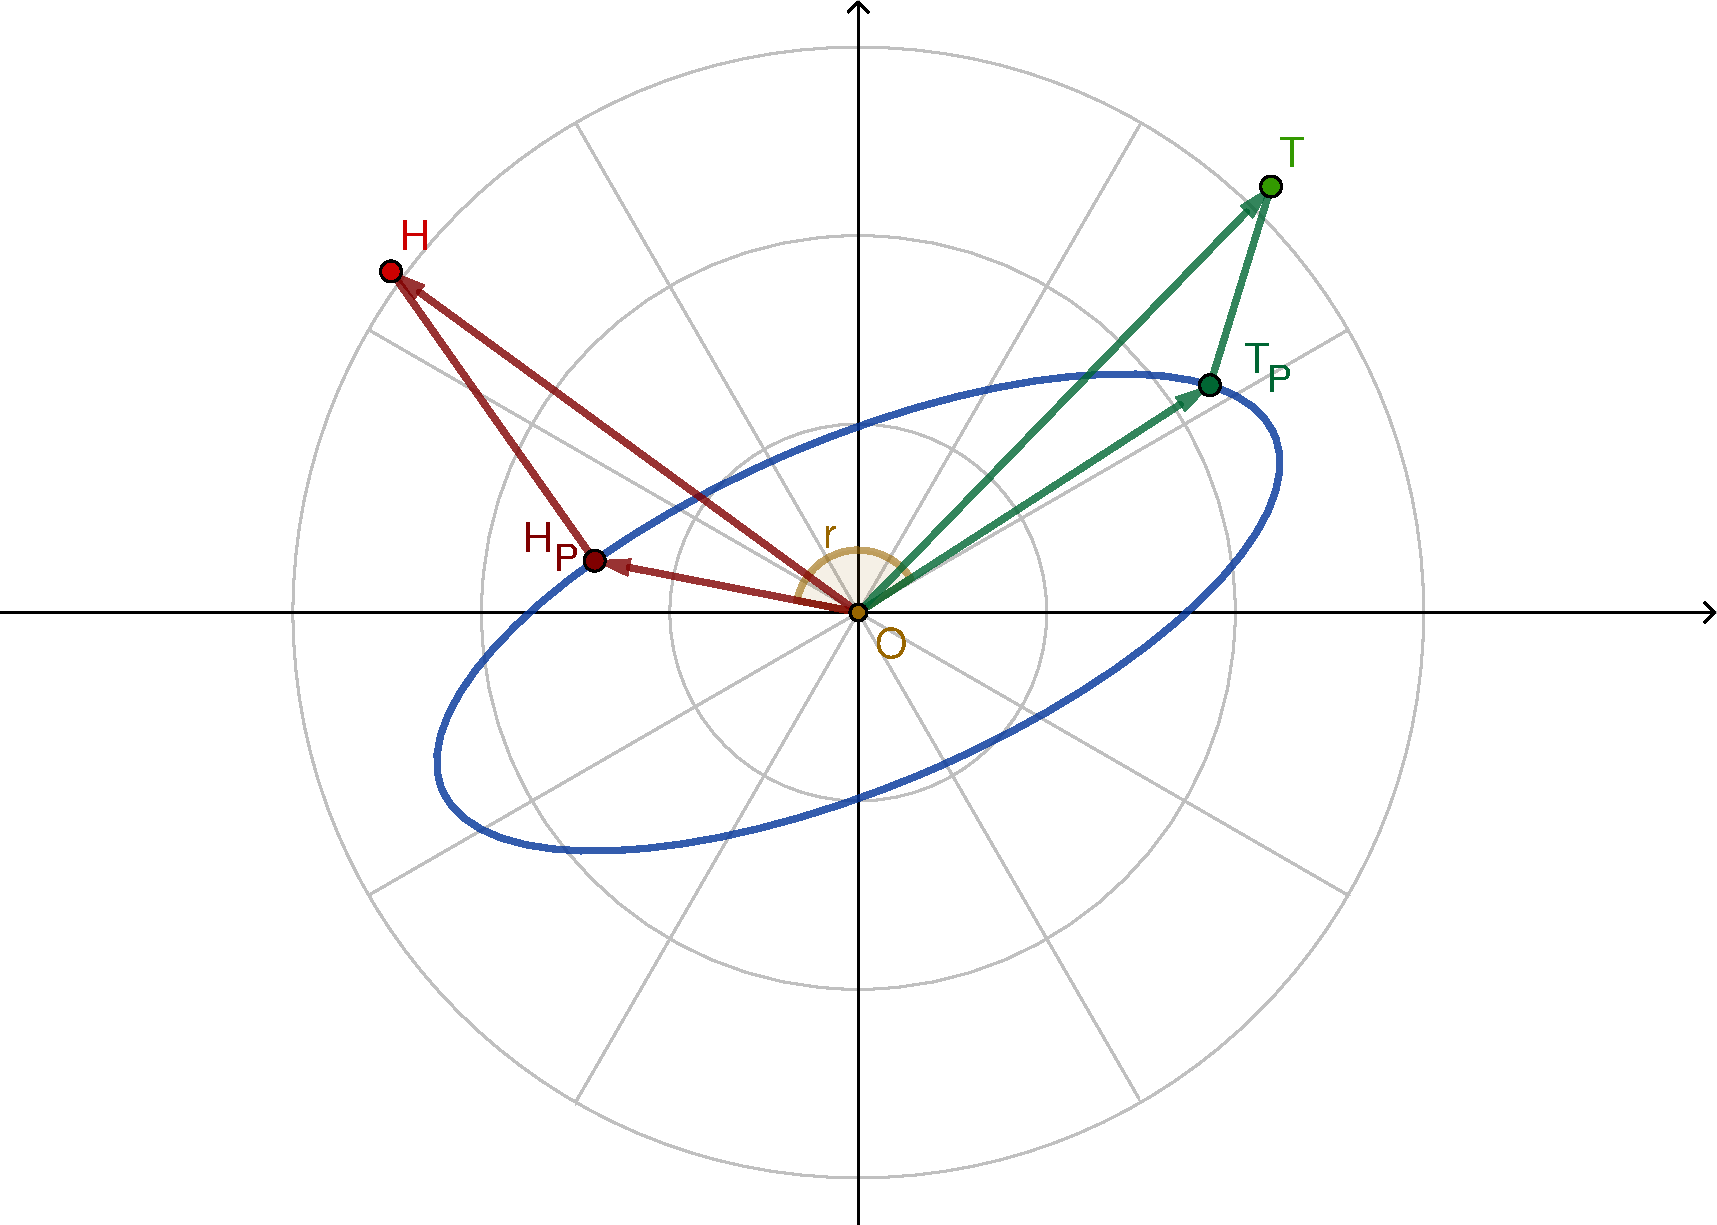
\includegraphics[width=0.4\textwidth,trim=0 0 0 0,clip]{figures/fig6.pdf}%trim裁切依次左下右上
	\vspace{0cm}
	\caption{图标题}
	\label{fig:pdf}
\end{figure}

\begin{figure}[!h]
	\centering
	\vspace{0cm}
	\includesvg[width=0.4\textwidth]{figures/fig5.svg}
	\vspace{0cm}
	\caption{图标题}
	\label{fig:svg}
\end{figure}

矢量图渲染速度要快得多,且效果更好。

\subsubsection{多张图片}
正文正文正文正文正文正文正文正文正文正文正文正文正文正文正文正文正文正文正文正文正文正文正文正文正文正文正文正文正文正文正文正文正文正文正文正文正文正文正文正文正文正文正文正文正文正文正文正文正文正文正文正文正文\cite{wiki,EM}正文正文正文正文正文正文正文正文正文正文正文正文正文正文正文正文正文正文正文如图\ref{fig:multi}所示

\begin{figure}[!h]
	\centering
	\subfigure[子图1标题]{
		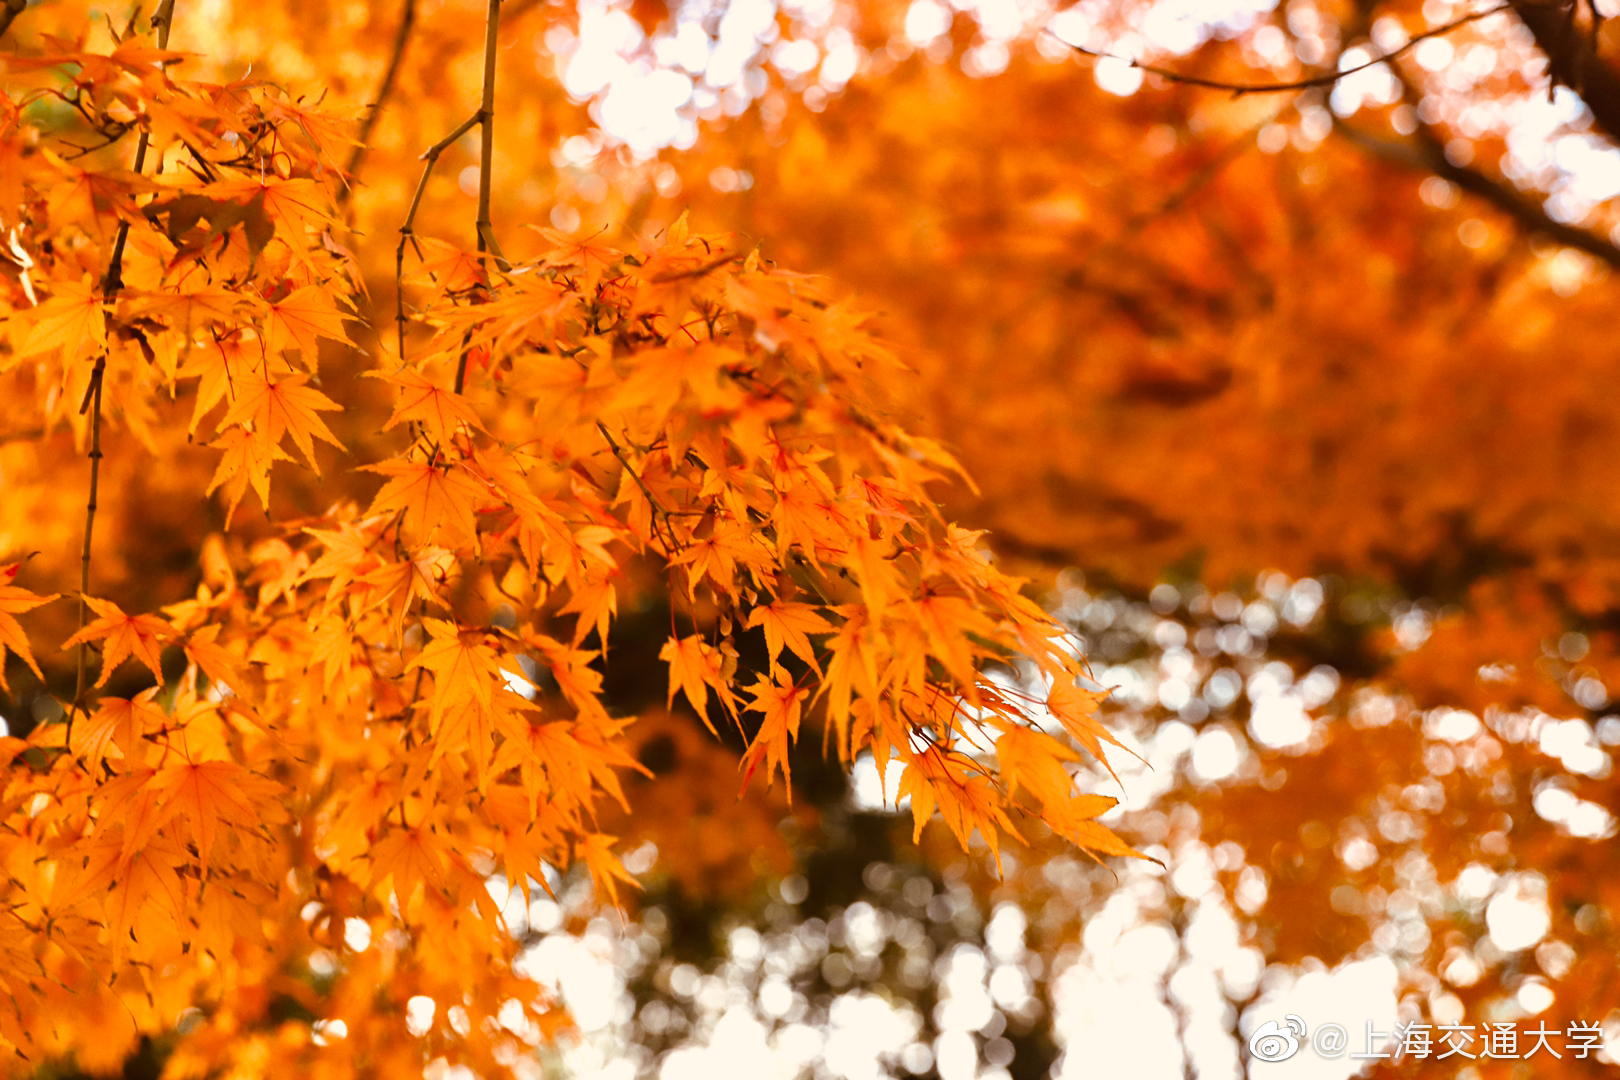
\includegraphics[width=0.2\linewidth,trim=0 0 0 0,clip]{figures/fig2-1.jpg}}%trim裁切依次左下右上
	\subfigure[子图2标题]{
		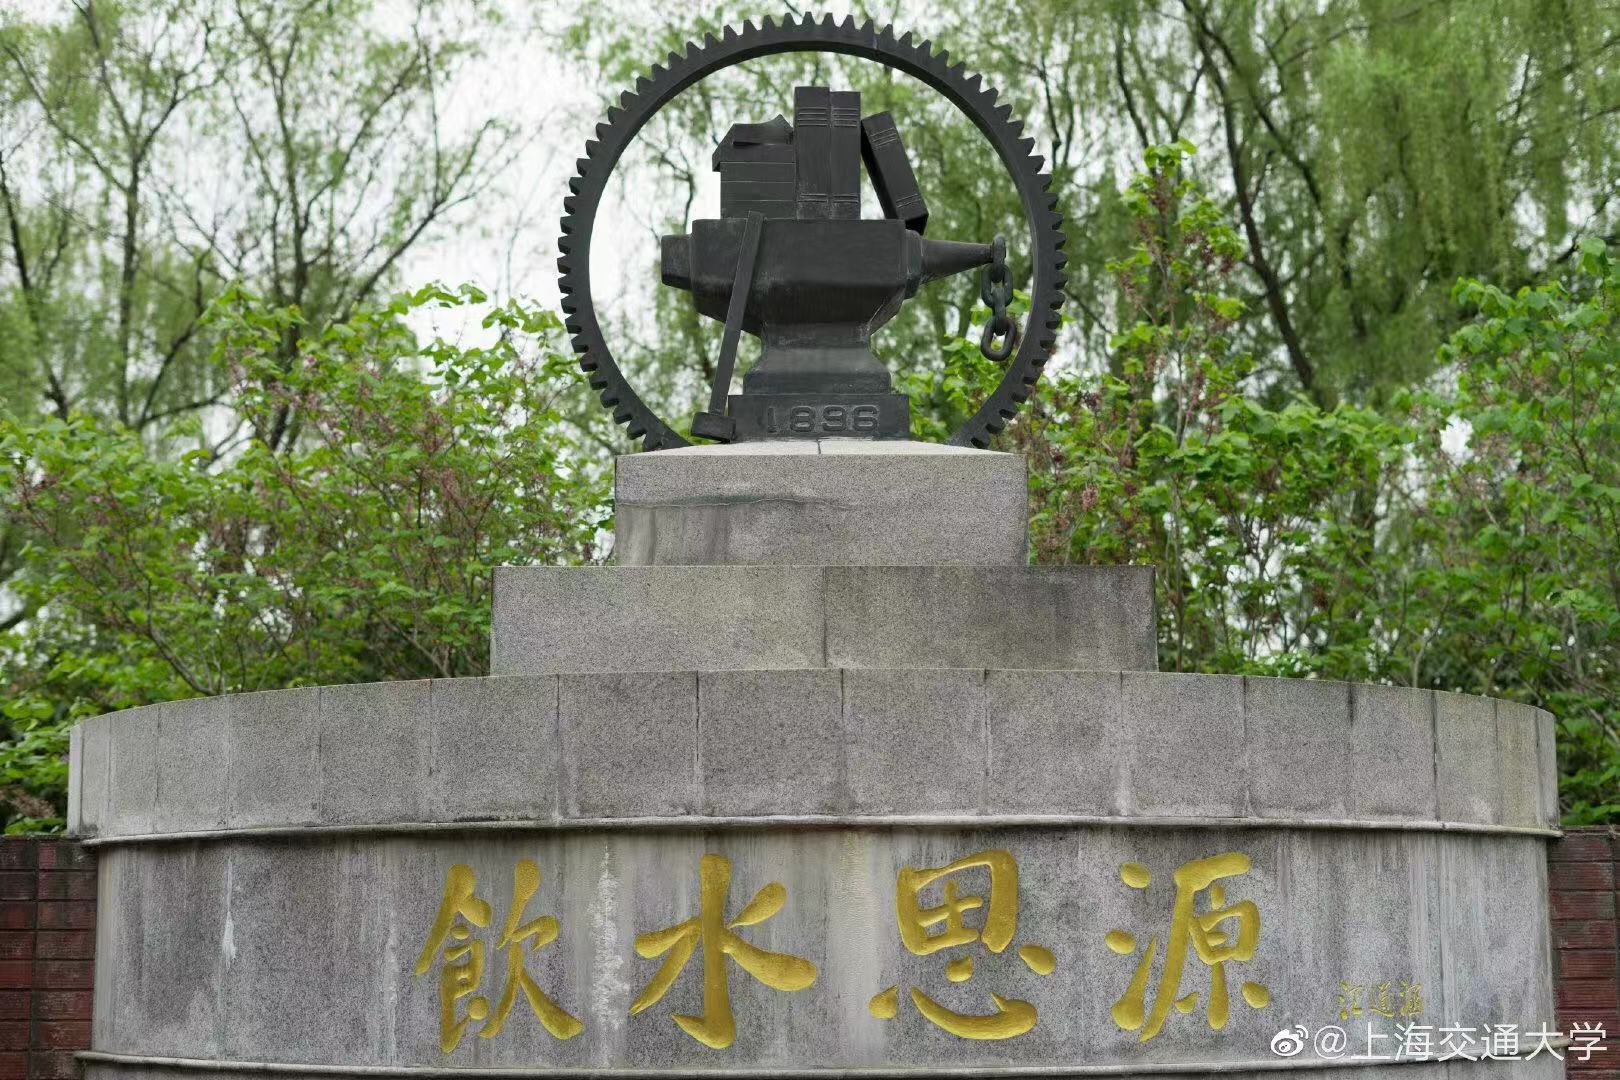
\includegraphics[width=0.2\linewidth,trim=0 0 0 0,clip]{figures/fig2-2.jpg}}%trim裁切依次左下右上
	\subfigure[子图3标题]{
		\includegraphics[width=0.2\linewidth,trim=0 0 0 0,clip]{figures/fig2-3.jpg}}%trim裁切依次左下右上
	\subfigure[子图4标题]{
		\includegraphics[width=0.2\linewidth,trim=0 0 0 0,clip]{figures/fig2-4.jpg}}%trim裁切依次左下右上
	\caption{图标题}
	\label{fig:multi}
\end{figure}
%多图并列换行自动,可用空格\quad等控制

\subsection{插入公式}
正文正文正文正文正文正文正文正文正文正文正文正文正文正文正文正文正文正文正文正文正文正文正文正文正文正文正文正文正文正文正文正文正文正文正文正文正文正文正文正文\textbf{行内公式}$1+1=2$正文正文正文正文正文正文正文正文正文正文正文正文正文正文正文正文正文正文正文正文正文正文正文正文正文正文正文正文正文正文正文正文

行间公式
$$
1-1=0
$$

更复杂的带序号行间公式见\ref{formula}
\begin{equation}
\begin{aligned}
1*1&=1\\
1/1&=1
\end{aligned}
\label{formula}
\end{equation}

完整公式汇总参见\url{https://1024th.github.io/MathJax_Tutorial_CN/#/document}

\newpage
\subsection{插入表格}

\begin{table}[!h]
    \centering
    \setlength\tabcolsep{3pt}
    \renewcommand{\arraystretch}{1.5}
    \begin{threeparttable}
        \begin{tabular}{ccccccc}
        \toprule
        % cmidrule 算0.几行
        \multirow{2.5}{*}{\makecell[c]{Model\\模型}}&\multicolumn {3}{c}{训练集^\dagger}&\multicolumn {3}{c}{开发集} \\
        \cmidrule(rl){2-4}\cmidrule(rl){5-7}
        &ACC&AUC&EER&ACC&AUC&EER  \\
        \midrule
        $GMM_{3}^{13}$&$0.9592$&$0.9393$&$0.0926$&$0.9596$&$0.9400$&$0.0911$\\    
        $GMM_{6}^{13}$&$0.9620$&$0.9506$&$0.0676$&$0.9623$&$0.9516$&$0.0654$\\ 
        $GMM_{9}^{13}$&$0.9659$&$0.9562$&$0.0592$&$0.9661$&$0.9564$&$0.0590$\\ 
        $GMM_{12}^{13}$&$0.9654$&$0.9543$&$0.0635$&$0.9654$&$0.9535$&$0.0646$\\ 
        $GMM_{15}^{13}$&$0.9654$&$0.9540$&$0.0641$&$0.9657$&$0.9551$&$0.0617$\\ 
        $GMM_{18}^{13}$&$0.9661$&$0.9560$&$0.0602$&$0.9661$&$0.9559$&$0.0603$\\ 
        \midrule
        $EGMM_{3}^{13}$&$0.9572$&$0.9474$&$0.0682$&$0.9569$&$0.9474$&$0.0677$\\    
        $EGMM_{6}^{13}$&$0.9621$&$0.9541$&$0.0587$&$0.9626$&$0.9553$&$0.0561$\\ 
        $EGMM_{9}^{13}$&$0.9632$&$0.9583$&$0.0495$&$0.9632$&$0.9585$&$0.0490$\\                         
        $EGMM_{12}^{13}$&$0.9619$&$0.9612$&$0.0399$&$0.9615$&$0.9604$&$0.0413$\\ 
        $EGMM_{15}^{13}$&$0.9629$&$0.9609$&$0.0423$&$0.9629$&$0.9606$&$0.0430$\\ 
        $EGMM_{18}^{13}$&$0.9630$&$0.9609$&$0.0425$&$0.9628$&$0.9606$&$0.0430$\\ 
        \bottomrule
        \end{tabular}
        \begin{tablenotes}
    	    \item[\dagger] 表格注释表格注释表格注释表格注释
        \end{tablenotes}
    \end{threeparttable}
    \caption{改变高斯分量数量结果对比}
    \label{table:demo}
\end{table}

表格\ref{table:todo}用于长文本自动换行
\begin{table}[!h]
    \centering
    \begin{tabular}{m{2cm}<{\centering} m{8cm}<{\centering} m{2cm}<{\centering}}
    \toprule
    问题重构 & 方案设计 & 时间规划 \\
    \midrule
    复现 & 使用PyTorch和SnnTorch等经过广泛验证的深度学习框架,完成基于MNIST等数据集的图像分类任务,与LeNet等进行对比,了解SNN的训练流程和原理 & 第8周\\ 
    \midrule
    迁移 & 构建更大的模型将SNN应用到目标检测等更为复杂的任务上 & 第11周\\ 
    \midrule
    探究 & 在上一步的模型基础上,通过设计对比实验,研究并验证SNN算法及特性 & 第12周\\ 
    \midrule
    融合 & 将SNN模型与ANN模型结合,通过可视化及数据验证,切实提高任务性能 & 第14周 \\ 
    \midrule
    展示 & 通过对网络层参数进行可视化,并利用训练输出绘制趋势图,对比实验结果 & 第16周 \\ 
    \bottomrule
    \end{tabular}
    \caption{脉冲神经网络相关研究规划}
    \label{table:todo}
\end{table}

\newpage
\subsection{插入伪代码}

\begin{algorithm}  
    \caption{基于广度优先搜索判断二分图}  
    \begin{algorithmic}[1] 
        \Require  强连通图$G$,上一轮调用时被遍历到的结点集$U$,及他们被归为的类$label$
          是否是二分图$Flag$
        \Function {IsBipartite}{$G,U,label$}
            \State $son\_of\_U\gets U$中结点的子结点
            \State
            \ForEach{$u\in son\_of\_U$}
            \If {$u\_label= label$}\algorithmiccomment{该结点已被归类且与其父结点相同}
            \State \Return{$Flag=False$}\algorithmiccomment{得到结果}
            \Else \If {$u\_label= -label$}\algorithmiccomment{该结点已被归类且与其父结点不同}
            \State $son\_of\_U\gets son\_of\_U - u$\algorithmiccomment{避免再次遍历该结点的子结点}
            \Else \algorithmiccomment{该结点未被归类}
            \State $u\_label\gets -label$\algorithmiccomment{将他们归为与其父结点不同的类}
            \EndIf
            \EndIf
            \EndForEach
            \State
            \If {$son\_of\_U=0$}\algorithmiccomment{所有的结点均已被归类}
            \State\Return{$Flag=True$}
            \Else \algorithmiccomment{归类在本轮被归类结点的子结点}
            \State \Return{\Call{IsBipartite}{$G,son\_of\_U,-label$}}
            \EndIf
        \EndFunction  
    \end{algorithmic}  
\end{algorithm}

\newpage
\subsection{插入代码}
\lstset{style=SQLStyle}
\begin{lstlisting}
SELECT name, course_id
FROM student, take as T
GROUP BY ID
HAVING COUNT(T.course_ID)>0;
\end{lstlisting}



\newpage
\section*{备注}
%Licence 请勿删除
本文排版基于\LaTeX{}\href{https://github.com/JamesZhutheThird/A-Simple-LaTeX-Template}{【Github】}\href{https://cn.overleaf.com/read/mxmypkyfrzpz}{【OverLeaf】}\href{https://latex.sjtu.edu.cn/read/ndjrkpksrfzn}{【SJTU-ShareLaTeX】}模板,采用\href{http://creativecommons.org/licenses/by-nc-sa/4.0/}{【CC BY-NC-SA 4.0】}进行许可。


\bibliographystyle{unsrt}
\bibliography{cite}

\appendix

\section{MATLAB代码}
\label{appcode:demo}
\lstinputlisting[language=matlab]{demo.m}

\section{表格和图片}
%%%
\setcounter{table}{0}   
\setcounter{figure}{0}
\renewcommand{\thetable}{B\arabic{table}}
\renewcommand{\thefigure}{B\arabic{figure}}
%%%以上四行需要针对每一个附录进行设置

代码引用参见\ref{appcode:demo},正文的图表编号是图\ref{fig:single}和表\ref{table:demo},附录的编号是图\ref{appfig:single}和表\ref{apptable:result},编号会重置。

\begin{figure}[!h]
	\centering
	\vspace{0cm}
	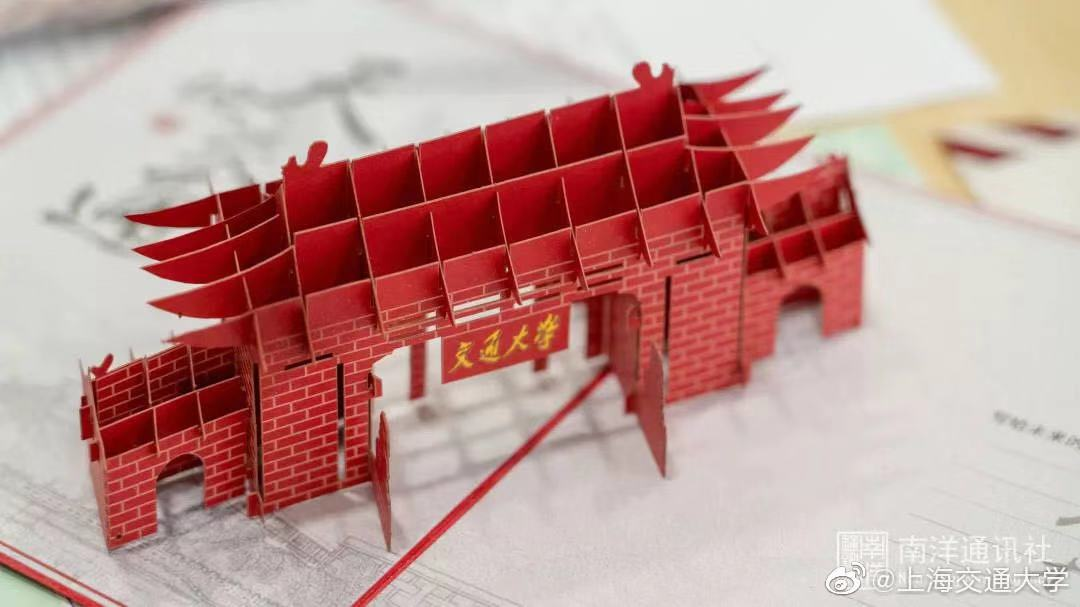
\includegraphics[width=0.4\textwidth,trim=50 100 200 75,clip]{figures/fig1.jpg}%trim裁切依次左下右上
	\vspace{0cm}
	\caption{图标题}
	\label{appfig:single}
\end{figure}

\begin{table}[!h]
    \centering
    \begin{tabular}{ccccccc}
        \toprule
        模型 & 训练集 $F1_{Micro}$ (最优Epoch) & 验证集 $F1_{Micro}$ & 测试集 $F1_{Micro}(Precision\&Recall)$  \\
        \midrule
        Linear & 62.324 (14k) & 62.285 & 62.960 ( 62.895 \& 63.025 ) \\
        Linear Nested & 62.002 (16k) & 61.875 & 63.766 ( 61.760 \& 65.905 ) \\ 
        CRF & 62.573 (15k) & 62.489 & 63.253 ( 63.967 \& 62.554 ) \\
        \bottomrule
    \end{tabular}
    \caption{不同模型性能对比}
    \label{apptable:result}
\end{table}

\end{document}
